\documentclass[10pt,letterpaper,onecolumn]{article}

\usepackage[left=1.0in,right=1.0in,top=1in,bottom=1in]{geometry}
\usepackage{amsmath,amssymb}
\usepackage[dvipdfmx]{graphicx}
\usepackage{acronym,etoolbox,color,multicol,xcolor}
%\usetikzlibrary{plotmarks}
\usepackage{subeqnarray,multirow,cite,array,setspace,fixltx2e,lineno,verbatim,mathtools,pgfplots,subfig}

\pgfplotsset{compat=newest}
\pgfplotsset{plot coordinates/math parser=false}
\newlength\figureheight
\newlength\figurewidth

\newcommand{\cmnt}[1]{\item}
\newcommand{\cmnts}[1]{\item[(#1)]}
\newcommand{\resp}{\item[\textit{\underline{Reply}}:]}

\newcommand{\mbf}[1]{\mathbf{#1}}
\newcommand{\me}[1]{\( #1 \)}
\newcommand{\mc}[1]{\mathcal{#1}}
\newcommand{\fall}{\forall}
\newcommand{\set}[1]{\left \lbrace #1 \right \rbrace }
\newcommand{\mvec}[2]{\mathbf{#1}_{#2}}
\newcommand{\ith}[1]{{#1}^\mathrm{th}}
\newcommand{\pr}[1]{{#1}^\prime}
\newcommand{\mbfa}[1]{{\boldsymbol{#1}}}
\newcommand{\herm}{\mathrm{H}}
\newcommand{\sset}[1]{\left [ #1 \right ]}
\newcommand{\rfrac}[2]{{}^{#1}/{}_{#2}}
\newcommand{\eqspace}{\IEEEeqnarraynumspace}
\newcommand{\enoise}{\widetilde{N}_0}
\newcommand{\eqsub}{\IEEEyessubnumber}
\newcommand{\eqsubn}{\IEEEyesnumber \IEEEyessubnumber*}
\newcommand{\neqsub}{\IEEEnosubnumber}
\newcommand{\review}[1]{{\textcolor[rgb]{0 0 0.6}{#1}}}
\newcommand{\trace}{\mathrm{tr}}
\newcommand{\tran}{\mathrm{T}}
\newcommand{\R}[1]{\label{#1}\linelabel{#1}}
\newcommand{\lr}[1]{page~\pageref{#1}, line~\lineref{#1}}
\newcommand{\eqn}[1]{\(#1\)}
\newcommand{\mx}{\mbf{m}}
\newcommand{\my}{\mbf{w}}
\newcommand{\mz}{\mbfa{\gamma}}
\newcommand{\mxb}{{{\mbf{m}}}}
\newcommand{\myb}{{{\mbf{w}}}}
\newcommand{\iterate}[2]{{#1}^{(#2)}}
\newcommand{\iter}[3]{{#1}_{#2}^{(#3)}}
\newcommand{\ma}{\mbf{x}}
\acrodef{MSE}{mean squared error}
\acrodef{IBC}{interference broadcast channel}
\acrodef{MC}{multi-cell}
\acrodef{BS}{base station}
\acrodef{MIMO}{multiple-input multiple-output}
\acrodef{SISO}{single-input single-output}
\acrodef{MU}{multiple-users}
\acrodef{OFDM}{orthogonal frequency division multiplexing}
\acrodef{WSRM}{weighted sum rate maximization}
\acrodef{QoS}{quality of service}
\acrodef{SCA}{successive convex approximation}
\acrodef{SNR}{signal-to-noise ratio}
\acrodef{MMSE}{minimum \acl{MSE}}
\acrodef{SIR}{signal-to-interference ratio}
\acrodef{SINR}{signal-to-interference-plus-noise ratio}
\acrodef{Q-WSRM}{queue \acl{WSRM}}
\acrodef{QM}{queue minimizing}
\acrodef{SRA}{spatial resource allocation}
\acrodef{JSFRA}{joint space-frequency resource allocation}
\acrodef{WMMSE}{weighted \acl{MMSE}}
\acrodef{KKT}{Karush-Kuhn-Tucker}
\acrodef{GP}{geometric programming}
\acrodef{SOC}{second-order cone}
\acrodef{BCDM}{block coordinate descent method}
\acrodef{ADMM}{alternating directions method of multipliers}
\acrodef{PD}{primal decomposition}
\acrodef{DD}{dual decomposition}
\acrodef{FFR}{fractional frequency reuse}
\acrodef{DC}{difference of convex}
\acrodef{Q-WSRME}{\ac{Q-WSRM} extended}


\DeclareGraphicsExtensions{{eps}}
\graphicspath{{Figures/}}
\renewcommand \thesection{\Roman{section}}
\renewcommand \thesubsection{\arabic{section}.\arabic{subsection}}

\renewcommand{\thefigure}{\Roman{figure}}
%\renewcommand{\thesubfigure}{\Roman{figure}}
\renewcommand{\theequation}{\roman{equation}}

\begin{document}


\usetikzlibrary{plotmarks}
\title{Reviewers Comments \& Authors Replies}

\date{}
\maketitle

\begin{tabular}{p{1.25in}p{4.25in}}
\textbf{Manuscript No.} & Paper T-SP-18051-2014, submitted to \emph{``IEEE Transactions on Signal Processing"} \\ \\
\textbf{Title} & ``Traffic Aware Resource Allocation Schemes for Multi-Cell MIMO-OFDM Systems" \\ \\
\textbf{Authors} & Ganesh Venkatraman, Antti T\"{o}lli, Markku Juntti, and Le-Nam Tran
\end{tabular}

\vspace{0.5in}
The authors would like to thank the associate editor and the reviewers for their valuable comments on the manuscript, which have been greatly helpful to improve the paper quality. Based on the comments, we have made several revisions to the paper, which are summarized below. 
\begin{enumerate}
	\item We have rewritten Appendix A-D to discuss the stationarity of limit points of the sequence of beamformer iterates generated by the centralized algorithms.
	\item We have updated the convergence of distributed algorithm to reflect the same.
\end{enumerate}

In what follows, the comments are listed, each followed immediately by the corresponding reply from the authors. The reviewers questions in the revised manuscript are highlighted in blue color and the authors responses are presented in black. Unless otherwise stated, all the numbered items (figures, equations, references, citations, etc) in this response letter refer to the revised manuscript. All revisions in the manuscript are highlighted in blue color.

\subsection*{List of Changes:}
\vspace*{1eM}
\begin{itemize}
	\item Page 6, paragraph after (28)
	\item Page 8, last paragraph in Section IV-B
	\item Page 12, paragraph following itemized requirements in Appendix A
	\item Last sentence after (51) on page 14
	\item Last paragraph in Appendix A-C
	\item Appendix A-D is rewritten using subsequence convergence
	\item Last sentence after (60) on page 15
\end{itemize}

Finally, to discuss the convergence of the sequence of iterates generated by the centralized scheme in Algorithm 1, we use an unified superscript index \eqn{t} to represent both \ac{AO} index \eqn{i} and \ac{SCA} indexing \eqn{k}. By doing so, we represent iterate \eqn{\mbf{x}^{t}} as the solution variable produced by the iterative algorithm in every \ac{SCA} \eqn{k} and \ac{AO} step {i}. Using this notation, we have revised our convergence discussions in Appendices A-C and A-D. 


\newpage
\section*{Response to Reviewer - \me{1}'s Comments}
In this paper, the authors proposed a traffic aware resource allocation scheme for multi-cell MIMO-OFDM systems, where the precoders at all BSs are chosen to minimize the total user queue deviations. The problem is nonconvex and the authors proposed two centralized algorithms based on the successive approximation (SCA) technique to find a stationary point. Moreover, several distributed algorithms are also proposed using primal decomposition, alternating directions method of multipliers (ADMM), and decomposition via KKT conditions, respectively.

Most sections of this paper are well written. The results and algorithms also seem valid. However, the motivation of minimizing the total user queue deviations is not well justified. The convergence results of some algorithms are not clearly presented. The presentation of the distributed solutions needs significant improvement. Analysis and comparison of the signaling overhead and computational complexity between the centralized and distributed algorithms are also necessary to justify the advantages of distributed algorithms.

\begin{itemize}

\cmnt{1} In Section II.B, please provides more justifications for the problem formulation in (6). For example, the Queue weighted sum rate maximization (Q-WSRM) is throughput optimal, i.e., if there exists a scheme which can make all queues stable, then the Q-WSRM can also do this. How about the proposed formulation in (6)? Is it also throughput optimal? 

\resp We thank the reviewer for the valid comment. The Q-WSRM scheme and the proposed schemes are all throughput optimal. It can be seen that the proposed extension Q-WSRME and the JSFRA formulations aims at minimizing the number of backlogged packets in addition to avoid the over allocation of the available resources. The JSFRA formulation with the \me{\ell_1} objective minimizes the number of backlogged packets in a greedy manner at each instant. By increasing the exponent \me{q \rightarrow \infty}, we obtain fair allocation at every transmission instant. We have included the discussions on the average number of backlogged packets at each instant for different arrival rates in Section V-C on page 13, col. 1. We have provided justifications for the problem formulation in (6) and (16) in page 5, col. 1, first paragraph.

\cmnt{2} Do the proposed solutions based on (6) achieve better average delay performance than the existing solutions? By the way, in the simulations, you should also add a figure comparing the average delay performance, instead of just comparing the performance metric defined by (6). This will better justify the advantage of the proposed solutions.

\resp The delay is proportional to the average number of backlogged packets in the queues. Moreover, delay depends on the service type. For example, if we consider a VOIP transmission, the delay requirement is stringent and can be achieved by increasing the priority factor \me{a_k} in (6a) using the current formulation. We can also address the fairness among the users by controlling the norm exponent \me{q} used in the objective function (6a). Since the current work is about the design of precoders to minimize the number of backlogged packets at each instant, we considered the residual number of backlogged packets as a performance measure.

\cmnt{3} In Section III.B, the convergence conditions under Algorithm 1 are not clear. First, you should be more specific about what is the SCA subproblem. Do you mean problem (19)? Second, does the uniqueness of the transmit and receive beamformers mean that the solution of the original problem in (16) is unique, or the solutions of the subproblems in (19) and (20) are unique, respectively?

\resp We understand the reviewer's point. We have updated the revised manuscript to discuss the convergence of the centralized algorithm in detail in Appendix B on page 14, col. 1. The discussions are provided for the convergence of the iterative algorithm. The uniqueness of the transmit and the receive beamformers are discussed in detail in Appendix B-C on page 15, col. 2.

\cmnt{4} It is better to clearly summarize the convergence conditions and results (i.e., does it converge to a stationary point or the optimal solution) for all algorithms in a theorem/proposition.

\resp The discussions on the convergence of the centralized algorithms are provided in Appendix B on page 14, col. 1 and for the distributed algorithms in Section IV-C on page 8, col. 2.

\cmnt{5} At the end of Section III, you mentioned that the proposed reduced complexity resource allocation scheme is sensitive to the order in which the subchannels are selected for the optimization problem. Please provide a discussion how to choose this order.

\resp We understand the reviewer's concern. Since the algorithm designs the precoders for each sub-channel at a time by using the total number of unserviced packets. For designing the precoders for the sub-channel \me{j+1}, we assume the transmit precoders and the rates of all users are obtained for the sub-channels \me{\{1,2,\dotsc,j\}}. Now, the number of backlogged packets for the \me{\ith{j+1}} sub-channel is given by 
\[Q_k - \sum_{i=1}^j \sum_{l=1}^L t_{l,k,i}\].
Since it depends on the rates of the already completed sub-channels \me{\{1,2,\dotsc,j\}}, it is susceptible to the ordering used to determine the precoders in each sub-channels. It is discussed in detail in Section III-D on page 7, col. 1.

\cmnt{6} In the distributed algorithms, it is not clear what exact information is exchanged between the BSs or between the BSs and users. Moreover, the signaling overhead should be analyzed and compared with the centralized solution. The proposed distributed algorithms require exchanging over-the-air signaling or backhaul signaling for many times within each channel coherent time (e.g., from Fig. 2, the distributed algorithm requires 20-30 iterations to converge even when there are only 3 subchannels). I don’t think this is acceptable in practice. Is the signaling overhead of the distributed algorithm really smaller than the centralized algorithm which only requires exchange the CSI between the BSs for once within each channel coherent time?

\resp Please note that the proposed distributed algorithm based on the primal or dual decomposition are discussed to approach to distribute the precoder design. Note that the distributed approaches are performed for the convex subproblem, which leads to the same stationary point asymptotically as that of the centralized solution. In reality, we have to limit the number of iterations required for each distributed algorithm, thereby leading to a point which may not be the same stationary point as when the algorithm is allowed to converge. In practice, we can combine the ADMM update, receiver update and the SCA update all at once to minimize the overhead in the backhaul signaling. We have provided a practical scheme in Section IV-D on page 9, col. 1. In a time-correlated channels, we can update the precoders once per coherence time when the number of backlogged packets are significantly large.

\cmnt{7} The convergence analysis of the distributed algorithms is not clear. For example, what is the exact condition to ensure the convergence of the distributed algorithms. Does the distributed algorithms also converge to a stationary point?

\resp We have updated the manuscript to include the discussions on the convergence of the distributed algorithm on page 8, col. 2 last paragraph in Section IV-C.

\cmnt{8} I’m totally confused with the ADMM approach in Section IV.A. Many notations, such as the local interference vector and consensus interference vector are used without formal definition. What is the difference between the local interference vector and consensus interference vector? What are their relationships with the actual interference vector. It seems that you are using the same notation for all of these interference vectors and I can’t tell when a notation refers to a local interference vector, a consensus interference vector, or the actual interference vector. These questions should be clarified and perhaps you should choose the notation system more carefully. For example, in (36), there are 3 similar notations and I don’t know which one is local interference vector and which one is the actual interference vector.

\resp We understand the reviewer's concern. We have shortened the section on ADMM by citing the relevant earlier work on the distributed implementation of the centralized algorithm for the min power problem [29]. We have rewritten the distributed algorithms in Section IV-A and Section IV-B. The variables are discussed in Section IV on page 8, col. 1. It follows the existing literature on the ADMM scheme, which treats the interference as a variable at each BS and the consensus on the interference is achieved upon convergence of the distributed algorithm as discussed in [11].

\cmnt{9} In the distributed algorithms, it is not clear what information is available at each node. For example, what are your assumption on CSIT (CSI knowledge at each BS) and CSIR (CSI knowledge at each user)? How to 2 obtain the information used to perform the required calculation at each node (such as calculating the actual interference, MMSE receiver and the dual variables)?

\resp We understand the reviewer's concern. For the distributed precoder design, we assume that the \ac{BS} \me{b} knows the channel \me{\mbf{H}_{b,k,n}} of all users in the system by the uplink sounding technique. Note that it includes the cross channel of the neighbor BS users as well. In addition, we assume the receivers are informed by the users by using precoded uplink pilots. We have included the information on what each network entity knows in page 7, col. 2 last paragraph. We have included the type of duplexing scheme adopted in the model, \textit{i.e}, TDD system, in the system description in Section II, last paragraph.

\cmnt{10} Do you have any convergence result for the proposed distributed solution based on the KKT conditions in Section IV.B? It seems that the iterative method to solve the KKT conditions is totally heuristic.

\resp We agree with the reviewer. Note that, if the dual variables are allowed to iterate until convergence, the proposed KKT based scheme achieves the same stationary point for each fixed receive beamformer (similar to the distributed algorithms). It is heuristic, since we update the transmit precoders, receive beamformers and the dual variables all at once in each iteration. Please note that the proposed algorithm is of practical significance, since it has few number of iterations before the actual transmission of data with the latest precoder update. It may not be a stationary point of the original nonconvex problem but it is guaranteed to provide better performance in the sum rate compared to the distributed approaches presented in Section IV-A and Section IV-B for the same number of iterations. We have provided additional details on the convergence of the KKT based approach in page 10, col 1, last paragraph.

\cmnt{11} Since queue is a dynamic system evolving according to (3), it doesn’t make sense to compare the queue deviations at a given time. You should compare average queue deviations in the simulations. Moreover, you should also compare the average delay performance instead of just comparing the performance metric (queue deviations) defined in this paper. Using the queue deviations as the performance metric also needs more justification.

\resp We thank the reviewer for raising the critical comment. Since the manuscript is about the precoder design to minimize the total number of backlogged packets in the system, we have provided the convergence behavior of the proposed precoder design formulations. The average queue deviation can be minimized by minimizing the deviations at each instant, we have provided the convergence plot for the single slot. In accordance with the reviewer comment, we have included the Section V-C on page 13, col. 1 to discuss the queue deviation over multiple transmission slots. We have presented Fig. 4a by comparing the average number of backlogged packets for different algorithms with various arrival bits and Fig. 4b for the number of backlogged packets at each instant. Please note that the delay is directly proportional to the number of backlogged packets if the arrivals are fixed, we are not addressing this explicitly. Even though, \me{\ell_2} and \me{\ell_{\infty}} norm addresses the delay and the fairness implicitly, we can prioritize the users with the weights \me{a_k} in (6a) for better service rate. We are currently working on the system level study of the proposed formulations.

\cmnt{12} What is “SRA” in the simulation figures?

\resp The \acf{SRA} is updated in the revised manuscript on page 7, col. 1, Section III-D.

\cmnt{13} In the discussion for Fig. 1, you mentioned that JSFRA converge to the optimal point, and all algorithms are Pareto-optimal. Since the problem is non-convex, why these algorithm can find optimal solution or Paretooptimal point? 

\resp We thank the reviewer for pointing out the mistake in the text. Since the problem is nonconvex, the JSFRA formulation can find a local optimal point upon convergence. The converged point of the JSFRA problem is in fact the stationary point of the original nonconvex problem, which is discussed in Appendix B-D on page 15, col. 2. We have removed the statement mentioning the pareto-optimal solutions in the discussions on Fig. 1 in the revised manuscript.

\end{itemize}


\newpage
\section*{Response to Reviewer - \me{2}'s Comments}
\review{The authors have addressed many of my previous comments. However, there are still several major issues that need further clarification.}

\vspace{1eM}
\underline{\textit{Reply:}} We thank the reviewer for providing useful comments. The comments are constructive and helped us to improve the manuscript better.

\begin{enumerate}

\cmnt{1} \review{The revised paper did not address my previous comment about how to select the sub-channel ordering. I understand that finding the best sub-channel ordering requires exhaustive search which has extremely high complexity. But it is important to provide a guidance on what would be a good choice of sub-channel ordering. For example, can we achieve a good performance by using a low complexity ordering algorithm such as a greedy sub-channel ordering algorithm?}

\resp We apologize for not discussing the sub-channel ordering in a detailed manner. We have included the guidelines for selecting the sub-channel ordering based on channel gains, \textit{i.e}, greedy selection. In random ordering scheme, after finding the precoders for a current sub-channel, we can choose any previously unselected sub-channels as the next candidate sub-channel for which the precoders are identified using the updated backlogged packets. As suggested by the reviewer, the greedy sub-channel ordering is based on sorting the best channel from each sub-channel, which is obtained by finding the highest channel norm between the users from the respective serving \ac{BS}. Note that the users channel used in the ordering procedure is the channel seen by the users with the corresponding serving \acp{BS} only.

However, it may not be optimal for all system configurations, since the ordering scheme should also consider the number of backlogged packets associated with each user. We have 
emphasized this issue by comparing various ordering schemes for the same system model with two different set of backlogged packets associated with each user. Even though we are not including it in the paper, we have included in the response letter to answer the reviewer's question. We considered a system with \eqn{N = 4} sub-channels, \eqn{N_B = 2} \acp{BS} with \eqn{N_T = 4} transmit antennas and \eqn{K = 12} single antenna users. The \ac{PL} is distributed uniformly over \eqn{[0,-3]} dB. The number of backlogged packets assumed for each user is provided in the corresponding captions in Fig. \ref{fig-review-1}.
\begin{figure*}[h!]
	\centering
	\subfloat[][Number of backlogged packets for each user in bits \eqn{Q_k = [11,8,14,6,6,2,10,10,5,6,9,5]}]{
		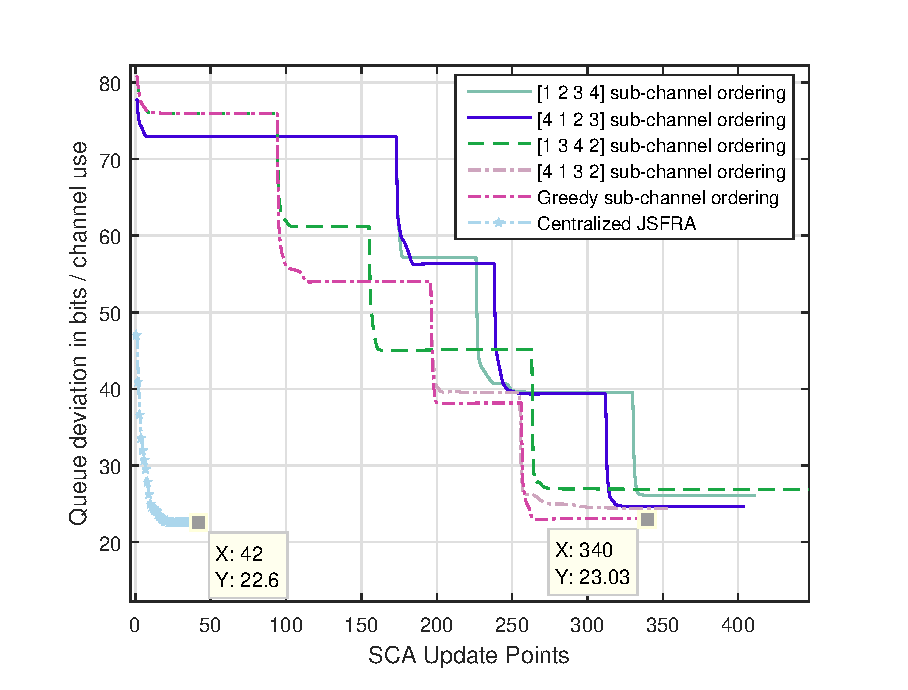
\includegraphics[width=0.8\textwidth]{reviewer_2_Q1B.eps}
		\label{fig-review-1a}
	}
	\hfill
	\subfloat[][Number of backlogged packets for each user in bits \eqn{Q_k = [8,9,12,8,12,5,4,10,8,5,7,9]}]{
		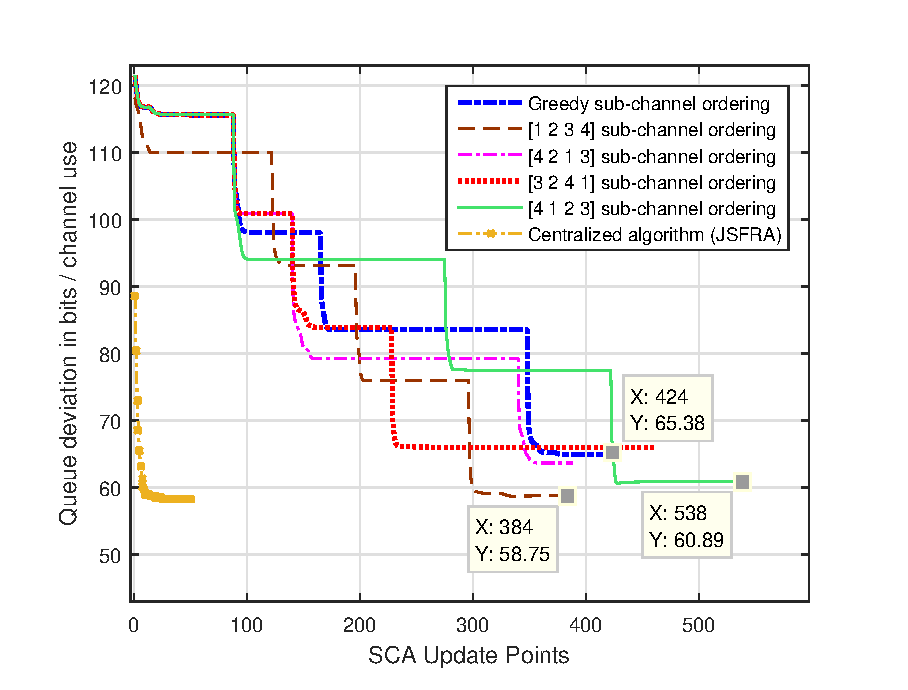
\includegraphics[width=0.8\textwidth]{reviewer_2_Q1A.eps}
		\label{fig-review-1b}
	}
	\caption{Convergence of the algorithms for \me{\lbrace N,N_B,K,N_T,N_R \rbrace = \lbrace 4,2,12,4,1 \rbrace} using \me{\ell_1} norm}
	\label{fig-review-1}
\end{figure*}

Fig. \ref{fig-review-1} compares different ordering of sub-channels with the total number of backlogged packets remaining in the system as the metric. As can be seen from Fig. \ref{fig-review-1a}, the greedy sub-channel ordering provides a favorable way of choosing the sub-channels to minimize the total number of backlogged packets. However in Fig. \ref{fig-review-1b}, the greedy sub-channel ordering is not an efficient strategy in determining the order in which the sub-channels are to be chosen. We have included the discussions regarding the greedy sub-channel ordering in the revised manuscript as a heuristic method under Section III-D final paragraph. Note that as the number of users in the system increases, all channel ordering provides favorable order to minimize the total number of backlogged packets in the system.

\cmnt{2} \review{The authors mentioned that the signaling overhead of the distributed algorithm can be reduced by using a smaller number of iterations \eqn{J_{\max}}. But still, you didn't answer my question about whether the signaling overhead of the distributed algorithm is smaller than the centralized algorithm. You should first analyze the signaling overhead of the distributed algorithm for fixed \eqn{J_{\max}} and the signaling overhead of the centralized algorithm. Then you should point out under what \eqn{J_{\max}} the distributed algorithm will have less signaling overhead than the centralized algorithm. Is it possible that the distributed algorithm always has more signaling overhead than the centralized algorithm even when \eqn{J_{\max} = 1}? Finally, there is a trade-off between performance and signaling overhead (\eqn{J_{\max}}) for the distributed algorithm. For the same signaling overhead (we can control \eqn{J_{\max}} to make the signaling overhead of the distributed algorithm approximately equal to that of the centralized algorithm), does the distributed algorithm achieve better performance than the centralized algorithm?}

\resp
	We thank the reviewer for the insightful comment and we apologize for the lack of clarity in explaining this information in our earlier manuscript.
	\begin{enumerate}
		\item The amount of signaling overhead of the distributed algorithm and the centralized one depends on the system model of consideration. For example, let us consider a model with \eqn{N = 1} sub-channels ,\eqn{N_B = 2} \acp{BS}, and \eqn{K = 4} users in total, each \ac{BS} serving \eqn{2} users. Let \eqn{N_T = 4} be the number of transmit antennas and \eqn{N_R = 1} be the number of receive antenna at each user. In this scenario, the amount of information exchange to perform a centralized algorithm by a common controller requires the knowledge of complete channel matrices interlinked in the system, \textit{i.e}, the number of users times the \acp{BS}. 
		
		In order to quantify the total number of bits required to be exchanged, let us assume that each complex channel for a single-input single-output requires \eqn{10} bits, \textit{i.e}, \eqn{4} bits for amplitude and \eqn{6} bits for phase (assuming phase is important) or it can be a equal share of \eqn{5} bits for both amplitude and phase. Using this assumption, the total number of channel information in bits to be exchanged via backhaul requires \eqn{10 \times K \times N_B \times N_R \times N_T = 320} bits. On the other hand, for the distributed case, let us consider \eqn{6} bits are required to quantize the scalar interference in the consensus vectors. Consequently, the proposed distributed solutions require \eqn{6 \times 2 \times 2} bits to be exchanged in each iteration. 
		
		In this example, for the same amount of signaling overhead as in centralized method, we can performance only up to 6 SCA updates for \eqn{J_{\max} = 2} (\textit{i.e.}, two updates for ADMM part). This may not be sufficient for the distributed algorithms to attain the same performance as the centralized method. However, as the number of sub-channels, users and/or the antenna element increases, it may not be a feasible option to feedback the \ac{CSI} across the coordinating \acp{BS} to the centralized controller. In addition to comparing the signaling overhead, we also need to consider the effects of the quantization of the \ac{CSI} on the performance of a centralized algorithm, which is beyond the scope of our paper. Generally, the performance is significantly degraded if the \ac{CSI} is quantized \cite{nam_robust}. Moreover, in the centralized algorithm, resulting transmit precoders need to be exchanged with the corresponding \acp{BS} before the actual transmission, involving huge overhead in the backhaul.
		
		\item Using the above discussion, we can say that when the system size is huge, it would be favorable to consider the distributed algorithm over the centralized approach due to the huge signaling overhead involved in exchanging the channels.
		
		\item In particular, \ac{ADMM} and primal approach requires significant overhead compared to the centralized algorithm for a small system, since by exchanging the quantized channels, each \ac{BS} can perform the centralized algorithm independently until convergence. However, it depends on the channel quantizer, which is likely to be based on the channel density function (eg. Lloyd quantizer). For a system involving more coordinating \acp{BS}, users and antenna elements, it would be beneficial to use distributed algorithm with \eqn{J_{\max} > 1} to have a strictly monotonic decrease in the objective. If we set \eqn{J_{\max} = 1}, the proposed algorithms still converge (but monotonicity of SCA is not guaranteed).
		
	\end{enumerate}
	
	We have included the above discussions in the first and last paragraphs of Section IV-C, and the paragraph before Section VI (i.e., the conclusion section). In reality, since the channel is time-correlated, it is enough to update the precoders once per radio frame. Thus, it is not necessary for the distributed algorithm to converge until the end. Instead, the decentralized parts only need to follow the fading process when \eqn{J_{\max} > 1}. 
	
	The performance of the distributed algorithm based on dual decomposition scheme was discussed for the time-correlated fading in Section C of [13], which shows that it is enough for the distributed precoder design to follow the fading process to provide desired performance. The distributed algorithm for the time correlated case is beyond the scope of our paper and thus is not considered in the current manuscript. However, we take this opportunity to show a plot demonstrating this behavior for the \ac{KKT} based algorithm presented in Section IV-C of the manuscript.
	\begin{figure}[h!]
		\centering
		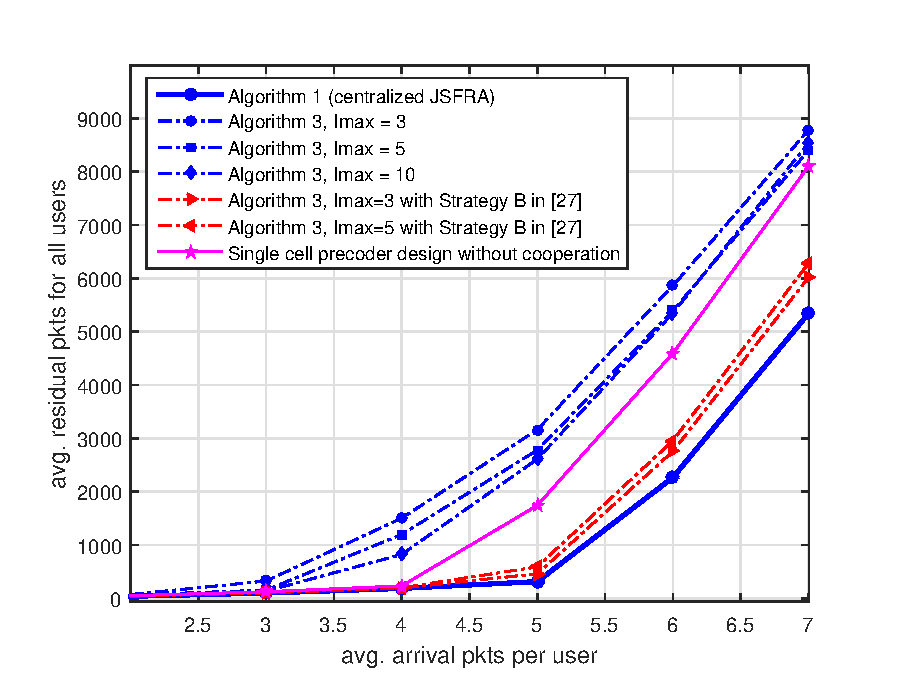
\includegraphics[width=0.8\columnwidth]{reviewer_2_Q2.eps}
		\caption{Average number backlogged packets after each transmission for system \me{\lbrace N,N_B,K,N_T,N_R \rbrace = \lbrace 4,2,16,4,2 \rbrace} evaluated for \eqn{500} slots}
		\label{fig-review-2}
	\end{figure}
		
	Fig. \ref{fig-review-2} compares the performance of the distributed \ac{KKT} approach presented in Section IV-C for different iteration. The signaling requirements are outlined in Algorithm 3 and the overhead involved in the signaling is penalized in the achievable rate of the users. We considered that the channel is coherent over \eqn{N_S = 100} symbols and the precoder update is performed by exchanging the equivalent channel for \eqn{J_{\max} = 3,5,10} number of iterations. The overhead is considered as \eqn{\tilde{t}_{l,k,n} = (1 - \frac{J_{\max}}{N_S}) \times t_{l,k,n}}, where \eqn{\tilde{t}_{l,k,n}} is the rate seen by the user and the factor \eqn{(1 - \frac{J_{\max}}{N_S})} is considered as a penalty involved due to the precoder exchange. The average number of backlogged packets after each transmission slot is evaluated as 
	\begin{equation}
	\chi = \sum_{k = 1}^K \; [ Q_k - \tilde{t}_k ]^+
	\end{equation}
	
	Unlike the distributed algorithm, the centralized scheme presented in Fig. \ref{fig-review-2} has no penalty term and it is used as a benchmark for the other figures. In order to improve the performance of the distributed scheme, the operating point involved in the \ac{SCA} algorithm is considered from the earlier frame instead of starting initializing randomly. Since we use \ac{KKT} approach, we can either use all users in the system for the precoder design or we can utilize single-cell MU-MIMO user selection presented in the literature to limit the number of users for which the precoders are designed, which leads to the faster convergence. As we can see from Fig. \ref{fig-review-2}, as the arrival rate per user increases, the performance of \ac{KKT} schemes with \eqn{J_{\max} = 3,5,10} converges since the number of backlogged packets are significantly large, therefore, the same set of users will be served by the algorithm with better precoders by utilizing the memory. 
	
	In spite of using memory and prior scheduling in the \ac{KKT} approach, isolated single \ac{BS} processing performs much better than the distributed scheme due to the limited number of iterations allowed in the algorithm. Note that the precoders are not updated for the desired users until convergence, after the limited number of iterations. However, if we perform the single cell precoder design by considering the neighboring precoders as fixed after the recent exchange as discussed in [28], we can improve the performance significantly for Algorithm 3 as shown by red curves in Fig. \ref{fig-review-2}. In this approach, in between each exchange across the coordinating \acp{BS}, each \ac{BS} will perform \eqn{J_{\max} = 20} with the neighboring precoders as fixed. Once the iterations are performed to update the precoders, it is then exchanged across the coordinating \acp{BS} to perform the same procedure as mentioned earlier. 

\cmnt{3} \review{If the authors can't prove the convergence of the ADMM algorithm (or the decomposition approach via KKT conditions) in Section IV.B, then at least, you should discuss the property of the fixed point of the algorithm. For example, does there exist a fixed point of the algorithm? If so, is the fixed point of the algorithm unique? Is any fixed point of the algorithm also the optimal solution of the original problem in (20)? Assuming that the ADMM algorithm converges to a fixed point, will the interference vector in (39) converges to the actual interference in the network? These questions must be clarified in the paper. Otherwise, it is not clear how the ADMM algorithm is related to the original problem in (20). Similar questions should also be answered for the decomposition approach via KKT conditions. }

\resp We thank the reviewer for raising the important concern regarding the convergence issue of the distributed algorithm with limited number of iterations. In view of this, we have updated the manuscript to include the discussion on the convergence of the distributed algorithms with a limited number of iterations in the third paragraph of Appendix B after (57). Since the distributed algorithm cannot be guaranteed to be monotonic in each iteration, it is not possible to prove the convergence of the algorithm. However, if the algorithm is allowed to converge or iterated to guarantee the monotonicity of the objective, it is possible to prove the convergence based on the discussions provided in the manuscript. 
\begin{itemize}
\item If there exists a fixed point or a set of fixed points for the original nonconvex problem in (16), then the proposed centralized algorithm in Section III-B and III-C finds at least one such point if iterated until convergence, which is provided in Appendix A. In order to find a unique fixed point, we regularize the objective function in (16) with a quadratic penalty term as discussed in Appendix A to transform the objective as a strongly convex function.
\item If the distributed algorithm is carried out for a limited number of iterations, it is not guaranteed to achieve a fixed point even if the outer \ac{SCA} update is performed for a large number of iterations. By this approach, the distributed approaches are not guaranteed to converge to a stationary point. In all our simulations on the primal and the \ac{ADMM} approach, we have set \eqn{J_{\max} = 20} in order to guarantee the monotonicity of the objective.
\item Unless the objective function is regularized with a strongly convex term as in Appendix A-C, the uniqueness of the iterates is not guaranteed. 
\item In each \ac{SCA} update, if the distributed algorithms are allowed to converge to the centralized solution, then the overall convergence will be a stationary point of the original nonconvex problem by following the same argument as that of the centralized algorithm.
\item Since the coupling between the distributed precoder designs is the interference between the BSs and the users, in the \ac{ADMM} approach, the interference is treated as a local variable, which is then included in the precoder design problem for each coordinating BS. This is treated as a local variable for individual \acp{BS}. Note that the local variable is an assumption made by the BS on the actual interference caused by the neighboring BSs. Since the actual interference caused is different, the consensus has to be made between the local interference variable maintained at each BS with the global consensus interference variable, which is nothing but the average between the corresponding BSs interference. These discussions have been made in the revised manuscript in Section IV-B. For reference purpose, we have also referred the interested reader to [11], which discusses exclusively about the ADMM approach. Upon convergence of the \ac{ADMM} approach, the interference vector is equal to the actual interference seen in the network.
\end{itemize}

\end{enumerate}

\bibliographystyle{./../../Styles/IEEEtran}
\bibliography{./../../Library/IEEEabrv,./../../Library/kirja_survey}


\newpage
\section*{Response to Reviewer - \me{3}'s Comments}
\textit{This manuscript focuses on the beamforming and scheduling optimization for IBC MIMO-OFDM system, including the centralized and decentralized optimization methods. This is an interesting and important topic.}

We thank the reviewer for reading the manuscript and providing valuable comments. The comments are really helpful in improving the manuscript.

\begin{itemize}

\cmnt{1} \textit{The number of transmitted packets \me{t_k}'s are optimization variables, which should be explicitly stated in the problem formulation of (6), (16), (19), (20) and (26) to avoid confusing.}

\resp Please note that the objective function uses \me{v_k =  Q_k - t_k = Q_k - \sum_{n = 1}^N \sum_{l = 1}^{L} \log_2(1+\gamma_{l,k,n})} expression instead of including an additional constraint for the transmitted packets using the rate expression and thus \me{t_k} is not a variable. However, in the MSE formulation, we have explicitly stated the optimization variable \me{t_k}, since it is present in the DC constraint (27).

\cmnt{2} \textit{The manuscript states that the inequalities (16b) and (16c) achieve equality at optimality(line 23, page 5). This is not obvious. An easy case to check this statement is that assuming the system has two BS and each BS serves one user. When \me{Q_1=0} and 2nd BS has sufficiently large power, (16b) and (16c) do not hold equality. Rigorous proof is needed if authors stick to this statement.}

\resp We thank the reviewer for the insightful comment. We have updated the manuscript to include the statement that the proposed approximation in (16b) and (16c) are the under estimator for the SINR expression in (2). The under estimator is tight when there is at least one user in each BS that cannot be served by the current transmission. It has multiple solutions, when the objective is zero even for a single BS. In this case, we can use a regularization term with the total power in the objective to obtain an unique solution. We have discussed the uniqueness of the proposed algorithm in detail in Appendix B-D.

\cmnt{3} \textit{The solution in (21) is obtianed for MMSE, i.e. for 2-norm(q=2). If \me{q=1} or \me{q=\infty}, it is actually an equivalent linear programming problem. Details for this solution should be provided.}

\resp We thank the reviewer for the critical comment. Note that the receiver has no explicit relation with the choice of \me{\ell_q} norm used in the objective function. The dependency is implicitly implied by the transmit precoders \me{\mvec{m}{l,k,n}}, which in deed depend on the \me{q} value. We have modified the text to included this information in page 5, col. 2, last paragraph.

\cmnt{4} \textit{The convergence proof need to be rigorous. The inequality of (23a) is opposite to the reference [28]. Also the statement on uniqueness of the transmit and the receive beamformers are not correct. Although we can choose one antenna to be real value, this does not mean the problem has unique solution!}

\resp We agree with the reviewer. We have updated the manuscript to discuss the convergence proof in a rigorous manner in Appendix B. The uniqueness is also justified implicitly by the linear approximation performed on the DC constraint (16b), which makes the transmit precoders to be susceptible to the phase rotation. The uniqueness discussions are presented in Appendix B-D.

\cmnt{5} \textit{(25) is generally wrong. (25) only holds when the MSE is minimized(by MMSE receiver) and the snr is the optimized(which is obtained by general eignvalue decompostion). This is clearly stated in the reference [5] and [6]. This can also be easily checked by comparing (25) and (2). Consequently the alternative formulation (26) based on this conclusion is questionable.}

\resp We agree that the MSE equivalence with the SINR expression is valid only when the receiver is based on MMSE objective. In our MSE reformulation solution, we have used the MMSE receiver irrespective of the \me{\ell_q} norm used in the objective. Since the receivers are based on the MMSE objective, the equivalence is valid between the MSE and the SINR expression. Since the transmit precoders are updated in accordance with the objective, the MSE reformulation yields the same solution as the SCA approach based JSFRA scheme presented in Section III-B. It can also be verified from Fig. 1 for \me{\ell_1} objective. We have updated the manuscript to include this comments on page 6, col. 2, line 10-13.

\cmnt{6} \textit{For ADMM aproach, the determination of the value of \me{\rho} in equation (35a) should be discussed. 1. The numbers of transmitted packets for users  \me{t_k}'s are optimization variables. So they should be explicitly stated in the problem formulation (6), (16), (20) and (26) to avoid confusing.}

\resp We agree with the reviewer's concern. We have included the reference [11] that discusses on the valid choices of the step size parameter for ADMM. We have included the statement that it depends on the system model under consideration. It is updated in the manuscript on page 8, col. 2, line 4-8.

\end{itemize}



\newpage
\section*{Response to Reviewer - \me{4}'s Comments}
This paper proposes a practical method for minimizing the number of currently backlogged packets in a wireless multi-cell MIMO-OFDM network. Resource allocation is performed over space (beamformers) and frequency (sub-carriers), and a norm of the queue deviations is minimized. The problem studied is very relevant, but still most work in the literature has so far focused on the infinite queue model which clearly does not reflect reality particularly well. The proposed methods seem practical, due to their possibility to be implemented as distributed methods coupled with distributed CSI acquisition. The paper has a multitude of approaches to the problem, but there are several areas which must be improved before a possible publication.

\vspace{0.1in}
\review{ First, we thank the reviewer for providing valuable and insightful comments. The comments are really helpful in improving the manuscript.}
\begin{enumerate}
\cmnt{1} {First, this reviewer is not convinced by the arguments for showing the convergence of the JSFRA method. "The SCA method" is often referred to, but never really defined or referenced. The three required conditions (as stated on p. 6, col. 1, rows 38-40) do not, as far as I can tell, appear in [27]. Indeed, [27] is concerned with optimization problems where the objective function is non-convex, but the constraint set is convex and separable over the blocks of variables. Perhaps you meant to cite [A], wherein non-convex constraints are handled in a similar way? Numerically, the algorithms do converge, and the argument put forward makes sense, but the treatment must be improved to be more rigorous.}

\resp \review{We agree that the original manuscript lacks the convergence proof for the JSFRA approach. We have presented a rigorous convergence proof for the proposed algorithm in Appendix B on the supplementary document. We have modified to include the reference suggested by the reviewer in [32] instead of [27], which is for the nonconvex objective function with the convex constraints.}

\cmnt{2} {Second, the optimization problems formulated only depend on $Q_k$, the current levels of backlogged packets, and not on the arrival rates. This is due to how the conditional Lyapunov drift is minimized. This approach completely removes the queue dynamics from the optimization problem, essentially leading to greedy one-shot optimization in every time instant. The framework would be more interesting if some sort of optimization (or tracking) is performed over several time instants, rather than the one-shot approach that is currently used for the JSFRA algorithms. Possibly, some expectation over the queues would be optimized then. Even if no analytical treatment of the tracking over several time-steps is added, I would at least highly recommend adding some simulation results where the proposed one-shot algorithms are performed sequentially over several time instants.}

\resp \review{
	\begin{enumerate}
	\item We thank the reviewer for the suggestion. In this paper, we proposed the precoder design to minimize the number of backlogged packets in the system at a given time. Since 
	the objective is minimized in each time instant, it minimizes the objective on an average as well.
	\item We focused on the design of the precoders based on the current knowledge of the channel state information in the system model. 
	\item As suggested by the reviewer, in order to justify the gains over multiple time instants, we have now included Section V-C with Fig. 4 to compare the performance of the JSFRA scheme for different \me{\ell_q} norm over multiple time slots. Plots comparing the average number of backlogged packets for different schemes at each instant and the number of queued packets remained in the system after each transmission instant are provided in Fig. 4.
	\end{enumerate}
}

\cmnt{3} {Third, the distributed methods (at least the primal decomposition and ADMM) seem to be fairly straight-forward applications of existing results. This reviewer recommends spending more space on the convergence, than on the description of the distributed techniques. Still, it would be nice with a direct description of what local CSI is required, and how it is acquired, to perform the local computations for the primal decomposition and ADMM methods. For the description of the signaling of the CSI in Sec. IV-B, are you envisioning a TDD system?}

\resp \review{
	\begin{enumerate}
		\item In accordance with the reviewer, we have shortened the discussions on the distributed approaches and discussed the convergence proof of the decentralized algorithm in Appendix C. 
		\item For the distributed precoder design, we assume that each \ac{BS} \me{b} knows the equivalent downlink channel \me{\mvec{w}{l,k,n}^\herm \mbf{H}_{b,k,n}} of all users in the system by using precoded uplink pilots, where the precoders are the MMSE receiver of all the users. Note that it includes the cross equivalent downlink channels of the neighbor BS users as well. To update the MMSE receiver, the equivalent channel for the \me{\ith{k}} user \me{\mbf{H}_{b,k,n} \mvec{m}{l,k^\prime,n}, \forall k^\prime \in \mc{U}_b, \forall b \in \mc{B}} is obtained from the BSs through user specific downlink precoded pilots. We have included the information on what each network entity knows in the paragraph after (36).
		\item We have included the type of duplexing scheme adopted in the model, \textit{i.e}, TDD system, in the system description in Section II, last paragraph.
		\end{enumerate}
	}

\cmnt{4} {Finally, some readers might be confused by the "joint space-frequency" terminology, believing that the beamforming is performed over a joint space-frequency channel space, where the space-frequency channels are formed by block-diagonal matrices, each block belonging to one sub-carrier. This could easily be clarified.} 

\resp \review{As per the reviewer's suggestion, we have clarified the space-frequency terminology in the lines before the last paragraph in Section I.}

\cmnt{5} {Please see the itemized questions}

\begin{enumerate}

\cmnts{a} - {p. 1, col. 1, row 42: "userss"}

\resp \review{Corrected in the revised manuscript in Section I first paragraph.}

\cmnts{b} - {p. 1, col. 2, row 18: the precoders are used \_implicitly\_ as decision variables. This is the whole point, to avoid explicitly modeling the hard decisions in the optimization, and instead do soft decisions during the iterations, and then finally hard decisions after convergence.}

\resp \review{We thank the reviewer for highlighting the insightful point. We have included the statement in the revised manuscript in Section I, second paragraph.}

\cmnts{c} - {p. 1, col. 2, row 33: Which chapter in [2] is referred to? With a quick look-through of the table of contents, I can't find and chapter or section treating the SCA method?}

\resp \review{We apologize for the inappropriate reference. We have updated the manuscript to include the proper reference on SCA with [22,32,34].}

\cmnts{d} - {p. 2, col. 2, row 36: Write $\text{rank}(.)$ and $\min$ instead}

\resp \review{We have updated the revised manuscript with the reviewer suggestions on the second paragraph in Section II.}

\cmnts{e} - {p. 3, col. 1, row 26: It would be more clear to explicitly write out the dependence of $\mathbf{M}$ and $\mathbf{W}$ in $\tilde{v}$ here}

\resp \review{We removed the matrix representation of the transmit precoders and the receive beamformers from the manuscript to avoid the confusion as suggested by the reviewer.}

\cmnts{f} - {p. 3, col. 2, row 26: Which general MIMO-OFDM problem are you talking about here, and what is combinatorial about it? Is it the problem of selecting users to be served on orthogonal subcarriers? There is nothing inherently combinatorial over the problem in (6) as far as I can tell, as the beamformers are used as soft decision variables.}

\resp \review{We thank the reviewer for pointing out the confusion. We have removed the word "combinatorial" from the text on the initial paragraph in Section III.}

\cmnts{g} - {p. 4, col. 2, row 40: "In fact, (5) provides similar expression of ..." This sentence is very hard to understand.}

\resp \review{We have rephrased the sentence to avoid difficulty in the understanding. The manuscript is updated with the revised text on the first paragraph in Section III.B.}

\cmnts{h} - {(16d): suggest your write out the power constraints here, in order to be faster be able to interpret the optimization problem. There is hardly any spaced saved by referring back to (6b).}

\resp \review{We have updated the manuscript with the explicit power constraint in (16d) as
\begin{equation}
\sum_{n = 1}^N \sum_{k \in \mathcal{U}_b} \sum_{l=1}^L \trace \, (\mvec{m}{l,k,n} \mvec{m}{l,k,n}^\herm) \leq P_{{\max}}, \fall b
\end{equation}}

\cmnts{i} - {p. 5, col. 1, rows 27-30: Here you might want to quickly mentioned how one could show the NP-hardness of (16).}

\resp \review{We have included the NP-hardness of the proposed solution by modeling the current problem to solve the \ac{WSRM} formulation, which is known to be NP-hard on the last sentence in Section III-B third paragraph.} 

\cmnts{j} - {p. 5, col. 1, row 50: "According to the SCA method...". I am not sure exactly how you define "\_the\_ SCA method"? Clarify or cite the definition.}

\resp \review{We have removed the sentence mentioning the SCA method. We have updated the manuscript to discuss this as SCA approach in the sentences after (17).}

\cmnts{k} - {p. 5, col. 2, row 31: Here is a case where it makes sense to reference earlier optimization constraints. However, are (19d) and (18) not the same??}

\resp \review{We thank the reviewer for pointing out the mistake. We have included all the constraints except the linearization constraint in (20), which is (19) in the original manuscript. Expression (19d) and (18) are the same. We have removed this double reference from (20).}

\cmnts{l} - {p. 5, col. 2, row 51: Slightly confusing with the notation between the iterates in (21b) and the MMSE filter in (22b).}

\resp \review{We have updated the manuscript to avoid the ambiguity in the representation of the optimal and the MMSE receiver. The optimal receiver is denoted by \me{\mvec{w}{l,k,n}^{o}} in (22) and the MMSE receiver by \me{\mvec{w}{l,k,n}} in (23).}

\cmnts{m} - {p. 6, col. 1, row 9: You might want to add somewhere that (22b) can be used instead of the fixed-point of (21b), since the scaling of the receive filters do not matter in the SINRs. However, does it affect the convergence of the algorithm?}

\resp \review{We thank the reviewer for the comment. We have updated the manuscript to include this discussion in the sentences after (23). The performance remains the same and the convergence rate is not affected by this scaling, which can be seen from Fig. 1 comparing the precoder convergence using the optimal and the MMSE receiver for the JSFRA scheme with \me{\ell_1} norm.}

\cmnts{n} - {p. 6, col. 2, rows 8-10: I don't fully understand the reasoning on the relation between the constraint sets in the different iterations. Why is this the case?}

\resp \review{To solve the nonconvex problem (16), we linearize the DC constraint (16b) around a fixed operating point. Since the operating point happens to be the optimal solution from the earlier iteration, the optimal point of the previous iterations is also present in the current feasible set. Therefore, at each iteration, the algorithm finds a better solution or the same compared to the previous solution, which leads to the monotonically decreasing objective. Please refer to Appendix B in the supplementary document for more details on the convergence analysis of the centralized algorithm.}

\cmnts{o} - {p. 7, col. 1, row 35: Just because a problem is convex does not mean that it has a unique solution. (Although it seems to me that (26) should have a unique solution.) Is the problem in (26) strictly convex?}

\resp \review{
	\begin{enumerate}
		\item We thank the reviewer for the critical comment. It is true that the convex problem need not required to have a unique solution in general. Using Minkowski inequality \me{\|x + y\|_q \leq \|x\|_q + \|y\|_q }, we can see that the JSFRA problem is not strictly convex for all exponents \me{\ell_q} used in the objective function. 
		\item The uniqueness of the solution is obtained due to the linear constraint (19) in the problem formulation (20). Note that the linear constraint (19) is susceptible to the phase rotations on the transmit precoders, whereas any unitary rotations on the transmit precoders still satisfies the original nonconvex constraint (16b). 
		\item When all the constraints (20) are active for all BSs, \textit{i.e}, when the objective is nonzero for all BSs, we obtain a unique set of transmit precoders. On the contrary, it has multiple solutions when the objective is zero even for a single BS. In this case, we can regularize the objective with a strictly convex term as
		\begin{equation}
		\|\tilde{\mbf{v}} \|_q + c \, \|\mbf{x} - \mbf{x}^{(i)}\|^2
		\end{equation}
		where \me{\mbf{x}} denotes the stacked vector of optimization variables and \me{\mbf{x}^{(i)}} denotes the value of \me{\mbf{x}} in the \me{\ith{i}} iteration. It is discussed briefly in the Appendix B-D. It makes the objective strictly convex, therefore, it has a unique minimum.
	\end{enumerate}
		}

\cmnts{p} - {Table 1: "backpreassure"}

\resp \review{It is updated in the manuscript in Table I.}

\cmnts{q} - {p. 11, col. 1, row 56: "performances". I'm not sure this is a countable noun.}

\resp \review{We thank the reviewer for pointing out the gramatical errors. We checked the gramatical validity and kept the plural in some cases.}

\end{enumerate}

\end{enumerate}

\end{document}
